%
% File NLP4MusA.tex
%
%% Based on the style files for NLP4MusA 2020, which were
%% Based on the style files for ACL 2018, NAACL 2018/19, which were
%% Based on the style files for ACL-2015, with some improvements
%%  taken from the NAACL-2016 style
%% Based on the style files for ACL-2014, which were, in turn,
%% based on ACL-2013, ACL-2012, ACL-2011, ACL-2010, ACL-IJCNLP-2009,
%% EACL-2009, IJCNLP-2008...
%% Based on the style files for EACL 2006 by 
%%e.agirre@ehu.es or Sergi.Balari@uab.es
%% and that of ACL 08 by Joakim Nivre and Noah Smith

\documentclass[11pt,a4paper]{article}
\usepackage[hyperref]{nlp4MusA}
\usepackage{times}
\usepackage{latexsym}
\usepackage{graphicx}
\usepackage{mathtools}  % amsmath with extensions
\usepackage{amsfonts}  % (otherwise \mathbb does nothing)
\usepackage{url}


%\aclfinalcopy % Uncomment this line for the final submission
%\def\aclpaperid{100} %  Enter the acl Paper ID here

%\setlength\titlebox{5cm}
% You can expand the titlebox if you need extra space
% to show all the authors. Please do not make the titlebox
% smaller than 5cm (the original size); we will check this
% in the camera-ready version and ask you to change it back.

\newcommand\BibTeX{B\textsc{ib}\TeX}


\title{Shift-Invariant Dictionary Learning using TCN-WTA Autoencoders for Discovering Musical Relations }

\author{First Author \\
  Affiliation / Address line 1 \\
  Affiliation / Address line 2 \\
  Affiliation / Address line 3 \\
  \texttt{email@domain} \\\And
  Second Author \\
  Affiliation / Address line 1 \\
  Affiliation / Address line 2 \\
  Affiliation / Address line 3 \\
  \texttt{email@domain} \\}

\date{}

\begin{document}
\maketitle
\begin{abstract}
Music temporal structure is full of shift-invariant patterns (e.g. motifs, ostinatos, loops, samples, etc.). In machine learning, the standard methods to encode a generic sequence is usually achieved by recurrent architectures such as LSTMs or Transformers. However, RNN architectures do not take advantage of this repetitive structure . We propose using a fully convolutional Temporal Convolutional Autoencoder to find a shift-invariant dictionary that can recreate symbolic multivariate musical signals. To find a dictionary we utilize a k-Winner Takes All (k-WTA) activation function to promote a sparse representation. In addition to gaining insight of shift-invariant patterns, some results indicate that CNN architectures can outperform recurrent networks on specific tasks and provide advantages while also demonstrating longer effective memory. We show few applications of this sparse representation such as de-noising musical ideas, unsupervised stylistic segmentation, and music generation. To assist related work, we have made interactive code available along with the trained models 


\end{abstract}

\section{Introduction}


The dictionary learning framework, requires using a few basis elements, atoms, learned from data itself. This appraoch has led to state-of-art results in various image and video processing tasks. Sparse dictionary learning has been successfully applied to various image, video and audio processing tasks as well as to texture synthesis[16] and unsupervised clustering.[Classification and clustering via dictionary learning ..] In evaluations with the Bag-of-Words model,\citep{Vogl2017} \cite{Koniusz2017} sparse coding was found empirically to outperform other coding approaches on the object category recognition tasks.

Sparse coding is a representation learning method which aims at finding a sparse representation of the input data (also known as sparse coding) in the form of a linear combination of basic elements as well as those basic elements themselves

There are multiple benefits in finding a sparse encoding of a signal. They can be used to encode prior knowledge in the sparsity patterns. Second, they are lightweight— requiring less memory to store and allowing faster inference and easier interpretability. Sparsity provides a way to discern patterns in an informed and principled manner, resulting in smaller model size . 
The ability to distil complex data structures such as music down to sets of dictionaries—salient features of a specific performer or music, has a multitude of applications in music. In our study, we are most interested in aiding music creation and ultimately building tools that take advantage of such ability. For instance, … [hint towards our applications]. 

\section{Related Work}


\subsection{ Dictionary learning  }
Given the data: $ X=\left[x_{1}, \ldots, x_{K}\right], x_{i} \in \mathbb{R}^{d} $ 
We want a dictionary $\mathbf{D} \in \mathbb{R}^{d \times n}: D=\left[d_{1}, \ldots, d_{n}\right]$ 
And a representation $R=\left[r_{1}, \ldots, r_{K}\right], r_{i} \in \mathbb{R}^{n}$ such that the reconstruction $\|X-\mathbf{D} R\|_{F}^{2}$ is minimized and $r_{i}$ are sparsed. The optimization problem can be formulated as: 

$\underset{\mathbf{D} \in \mathcal{C}, r_{i} \in \mathbb{R}^{n}, \lambda>0} {\operatorname{argmin}} \sum_{i=1}^{K}\left\|x_{i}-\mathbf{D} r_{i}\right\|_{2}^{2}+\lambda\left\|r_{i}\right\|_{0}$ \\   $\mathcal{C} \equiv\left\{\mathbf{D} \in \mathbb{R}^{d \times n}:\left\|d_{i}\right\|_{2} \leq 1 \forall i=1, \ldots, n\right\} $
\\ \\
However this formulation does not look for shift invariant features. 

\subsection{ Shift-invariant dictionary learning (SIDL)  }

In previous works, various shift-invariant dictionary learning (SIDL) methods have been employed to discover local patterns that are embedded across a longer time series in sequential data such as audio signals. While \cite{Grosse2007} employs shift-
invariant sparse coding with a convolutional optimization and gradient descent method for an audio classification task, \cite{Zheng2016} demonstrates an efficient algorithm with the ability to combine shift-invariant patterns in a sparse coding of the original data for audio reconstruction and classification tasks. Such unsupervised learning methods have shown to be powerful in discovering shift-invariant patterns and a handful of studies have implemented SIDL for the purpose of music. Although music transcription and classification tasks have seen a strong usage of sparse dictionary learning in the past [Shift-Invariant Sparse Coding for Audio Classification, NMF based Dictionary Learning for Automatic Transcription of Polyphonic Piano Music, Sparse and Shift-Invariant Representations of Music, Music Genre Classification using On-line Dictionary Learning, Learning Sparse Dictionaries for Music and Speech Classification, Context-Dependent Piano Music Transcription With Convolutional Sparse Coding], we have yet to see a study that harnesses the advantages of sparse representation for the purpose of music creation. Instead, the popular methods for discovering music relations and achieving music generation have been a transformer with some sort of attention mechanism or the recurrent architectures. [Discovering Music Relations with Sequential Attention], for instance, uses an attention module that is tailored to the discovery of sequence level relations in music, while studies like \cite{Roberts2018} uses the recurrent variational autoencoder and a hierarchical decoder in order to model long-term musical structures. 




\subsection{Temporal Convolutional Networks (TCN) }
 Some of the most notable benefits include longer effective memory and low memory requirement when training. We explore these benefits for the purpose of music, which inherently requires a longer history due to musical temporal structure. Moreover, the low memory requirement of the convolutional architecture combined with a sparse representation in dictionary learning presents a strong potential for lighter and faster modeling with a high prospect of being applied to a real-time and on-line dictionary learning in the future. In this paper, we propose SIDL using TCN WTA-Autoencoders for discovering music relations—salient features of a specific performer or music, and illustrate potential applications in music analysis and creation. Some Benifits of TCN over RNNs are Parallelism, flexible receptive field size, and low memory requirement for training


\subsection{SIDL by TCN K-WTA Autoencoders}

In our study, we use a fully convolutional temporal autoencoder to find shift-invariant dictionaries while ensuring sparsity via the K-WTA activation function [Winner-Take-All Autoencoders]. The use of K-WTA in conjunction with dictionary learning was inspired by [Towards Contrastive Learning for Time-Series] where the K-WTA’s ability to achieve sparse representations is explored in the context of constructive learning for time-series data. The use of Temporal Convolutional Nets was encouraged by various advantages that convolutional architectures bring for sequence modeling over recurrent networks as illustrated in \cite{ShaojieBai2018}.



\section{Experiments}
\label{ssec:experiments}

We show a few applications of our TCN k-WTA model 

\begin{itemize}
\item Cleaning musical sections
\item Unsupervised feature extraction 
\item Generating new music
\end{itemize}


\subsection{Datasets}
\label{ssec:experiments}

We use two distinct datasets: MAESTRO  \cite{hawthorne2018enabling}, and  grove Groove  \cite{groove2019} . See table 2 for more details on the datasets used. We also use distinct MIDI representations for each dataset. 

\begin{table*}[ht]
    \centering
    \begin{tabular}{p{0.15\linewidth} | p{0.15\linewidth} | p{0.1\linewidth}  | p{0.45\linewidth} }
      Dataset  & Size  & Instrument &  MIDI Representation\\ \hline
      MAESTRO  & 1020 (Hrs)   & Piano &  One-hot encoding over 388 different MIDI events. Every datapoint here has an arbitrary length \\
        \hline
        Groove & 3.6 (Hrs)  & Drum &  T timesteps (one per 16th note) and 27 MIDI events. We use fixed length 64 time step sections\\
    \end{tabular}
    \caption{Datasets used to experiment with fully convolutional temporal autoencoder model. All datasets used are MIDI format }
    \label{tab:my_label}
\end{table*}

\subsection{Model Implementation}
Our model implementation differs slightly for the different datasets used. 

\begin{figure}[ht]
  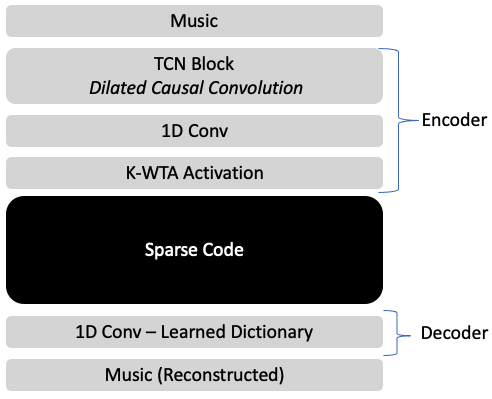
\includegraphics[width=\linewidth]{/Users/juanhuerta/personal_projects/code/shift_invariant_dictionary_learning/paper/images/tcn.png}
  \caption{After training the model we can use it to encode datapoints of arbitrary length unsupervised stylistic segmentation. We use PCA on the average sparse code for each piece. We project into 2 dimensional sparse to visualize }
  \label{fig:boat1}
\end{figure}

\textbf{MAESTRO} 
\\
Our TCN-KWTA Autoencoder is designed with [1, 8, 16, 32, 1000, 1] layers. The sparse representation is the layer before the last. Our WTA activation function is in the layer before the last. We also use a decaying WTA activation fucntions
\\
\begin{figure*}[ht]
  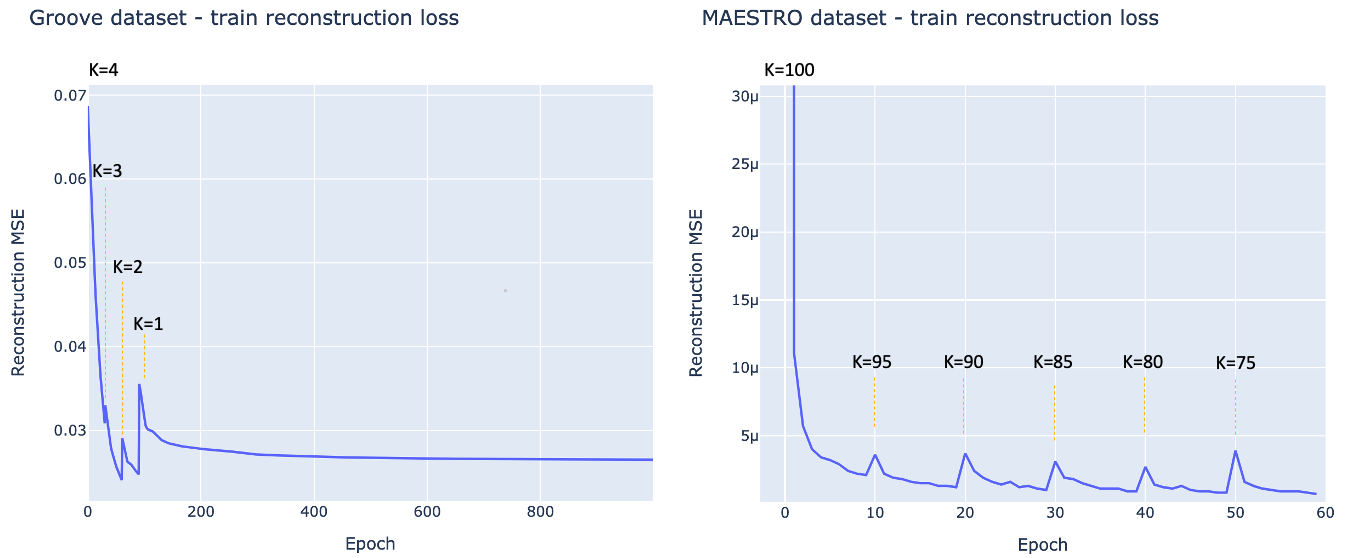
\includegraphics[width=\linewidth]{/Users/juanhuerta/personal_projects/code/shift_invariant_dictionary_learning/paper/images/maestro.png}
  \caption{After training the model we can use it to encode datapoints of arbitrary length unsupervised stylistic segmentation. We use PCA on the average sparse code for each piece. We project into 2 dimensional sparse to visualize }
  \label{fig:boat1}
\end{figure*}

\textbf{GROOVE} 
\\
Our TCN-KWTA Autoencoder is designed with [1, 8, 16, 32, 1000, 1] layers. The sparse representation is the layer before the last. Our WTA activation function is in the layer before the last. We also use a decaying WTA activation fucntions


\subsection{Music Reconstructions}
\label{ssec:first}

Center the title, author's name(s) and affiliation(s) across both
columns. Do not use footnotes for affiliations. Do not include the
paper ID number assigned during the submission process. Use the
two-column format only when you begin the abstract.

The title, author names and addresses should be completely identical
to those entered to the electronical paper submission website in order
to maintain the consistency of author information among all
publications of the conference. If they are different, the publication
chairs may resolve the difference without consulting with you; so it
is in your own interest to double-check that the information is
consistent.

\subsection{Keep Top N Dictionary words }

Another application of having a sprase code, is the ability to recognize the most used words in the dictionary. Given a sparse code we can limit a piece to only be made up of the top N words. Some example applications of keeping to top N words are for example, low dimensionality feature extraction for machine learning taks; music reduction--reduction wherein the complexity of the arrangement is reduced to a simpler transcription and parts. And Music Segmentation (Discretization) wherein various musical ideas used in a piece of music are isolated from the piece itself. Such segmented ideas could be used in analysis or creatively repurposed to generate new music.

\subsection{Unsupervised Stylistic Segmentation }
\begin{figure*}[ht]
  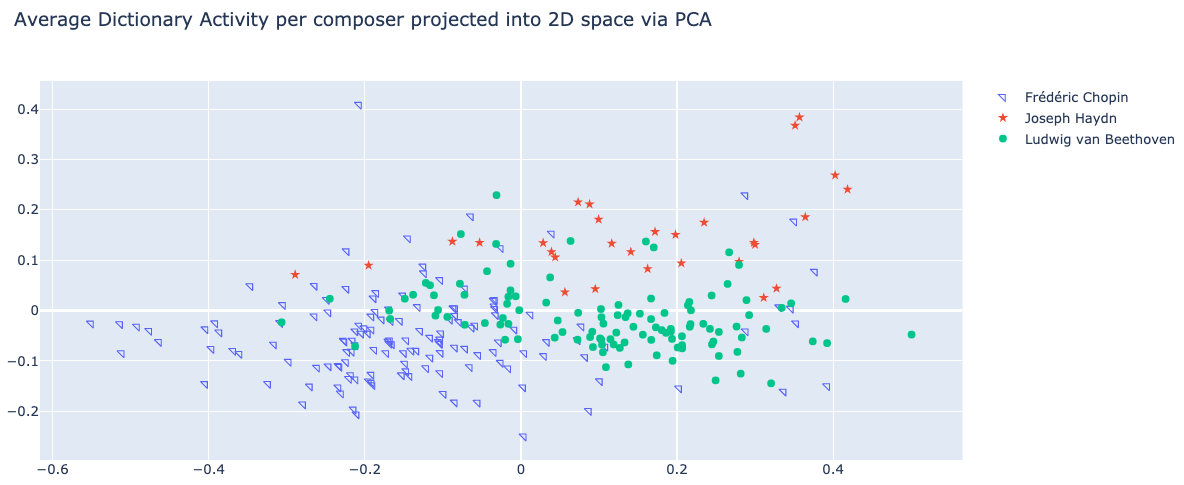
\includegraphics[width=\linewidth]{/Users/juanhuerta/personal_projects/code/shift_invariant_dictionary_learning/paper/images/newplot.png}
  \caption{After training the model we can use it to encode datapoints of arbitrary length unsupervised stylistic segmentation. We use PCA on the average sparse code for each piece. We project into 2 dimensional sparse to visualize }
  \label{fig:boat1}
\end{figure*}



If we train with a dataset that includes multiple composers we should expect to find that different composers utilize different shift invariant patters. To visualize kernel usage we average out the rows of our sparse code. This should provide us with the average dictionary word value. If we do PCA on the average dictionary vector and reduce dimensionality to 2D. We obtain the plot in Figure 2

It is also possible to use this average kernel usage for each composer and make comparisons for composers, such as most similar or disimilar between styles or comparisons. 


\subsection{Genrating Structured Drums}

If we have a specific musical structure we would like to follow. For example, 4/4 120bpm. We can train inject prior information into our 1D convolutions. For example, we can make each kernel the length of 1/4 beat. This allows for better dictionary learning since repetition is expected to happen at this time steps. We can stitch together musical sections, to create bars of music. and desing a specfic structure 



%% NOTE: NLP4MusA desn't need DOI.
% BEGIN: remove
% \textbf{Digital Object Identifiers}:  As part of our work to make ACL
% materials more widely used and cited outside of our discipline, ACL
% has registered as a CrossRef member, as a registrant of Digital Object
% Identifiers (DOIs), the standard for registering permanent URNs for
% referencing scholarly materials.  As of 2017, we are requiring all
% camera-ready references to contain the appropriate DOIs (or as a
% second resort, the hyperlinked ACL Anthology Identifier) to all cited
% works.  Thus, please ensure that you use Bib\TeX\ records that contain
% DOI or URLs for any of the ACL materials that you reference.
% Appropriate records should be found for most materials in the current
% ACL Anthology at \url{http://aclanthology.info/}.
%
% As examples, we cite \cite{P16-1001} to show you how papers with a DOI
% will appear in the bibliography.  We cite \cite{C14-1001} to show how
% papers without a DOI but with an ACL Anthology Identifier will appear
% in the bibliography.  

%  As reviewing will be double-blind, the submitted version of the papers
%  should not include the authors' names and affiliations. Furthermore,
%  self-references that reveal the author's identity, \emph{e.g.},
%  \begin{quote}
%  ``We previously showed \cite{Gusfield:97} ...''  
%  \end{quote}
%  should be avoided. Instead, use citations such as 
%  \begin{quote}
%  ``\citeauthor{Gusfield:97} \shortcite{Gusfield:97}
%  previously showed ... ''
%  \end{quote}

% Any preliminary non-archival versions of submitted papers should be listed in the submission form but not in the review version of the paper. NLP4MusA reviewers are generally aware that authors may present preliminary versions of their work in other venues, but will not be provided the list of previous presentations from the submission form. 
% END: remove


\subsection{Genrating Piano Music }

Type the abstract at the beginning of the first
column. The width of the abstract text should be smaller than the
width of the columns for the text in the body of the paper by about
0.6 cm on each side. Center the word \textbf{Abstract} in a 12 point bold
font above the body of the abstract. The abstract should be a concise
summary of the general thesis and conclusions of the paper. It should
be no longer than 200 words. The abstract text should be in 10 point font.





\section{Discussion}
\label{ssec:discussion}

There are multiple benefits to this sequence learning methodology. The first is such as simplicity and felxibilty, the TCN autoencocoder is a simple to implemnt arquitecture and requires any abitrary size combinations of multivariate musical signals.Also the size of the model for both Magenta and Groove are 877 KB and 750 KB respectively. In comparison, googles Performance RNN--LSTM-based recurrent neural network--is ~25MB, and other transformer based models can be GBs in size. 

In addition, our method allows for incorporating known structural information into a model prior to trainng. and finally we have the most imporant benifit is the sparse representatoin and learned dictionaries, as we have shown this can be used for mutiple applications and analysis. 

The performance on the recustruction and generation on for the drum Grove dataset  was significantly better than the piano (MAESTRO dataset). This is in part because the dataset was pre-proccessed to match with kernel size, and the drum sections were the same length and have lower dimensionality. 



% Min: no longer used as of ACL 2019, following ACL exec's decision to
% remove this extra workflow that was not executed much.
% BEGIN: remove
%% \section{XML conversion and supported \LaTeX\ packages}

%% Following ACL 2014 we will also we will attempt to automatically convert 
%% your \LaTeX\ source files to publish papers in machine-readable 
%% XML with semantic markup in the ACL Anthology, in addition to the 
%% traditional PDF format.  This will allow us to create, over the next 
%% few years, a growing corpus of scientific text for our own future research, 
%% and picks up on recent initiatives on converting ACL papers from earlier 
%% years to XML. 

%% We encourage you to submit a ZIP file of your \LaTeX\ sources along
%% with the camera-ready version of your paper. We will then convert them
%% to XML automatically, using the LaTeXML tool
%% (\url{http://dlmf.nist.gov/LaTeXML}). LaTeXML has \emph{bindings} for
%% a number of \LaTeX\ packages, including the ACL 2019 stylefile. These
%% bindings allow LaTeXML to render the commands from these packages
%% correctly in XML. For best results, we encourage you to use the
%% packages that are officially supported by LaTeXML, listed at
%% \url{http://dlmf.nist.gov/LaTeXML/manual/included.bindings}
% END: remove

\section{Conclusion}

We have shown that TCN-kWTA autoencoder can learn a sparse representation of abitrary length musical signal. This shift invariant, sparse representation can be used to analyze, preprocess, or generate musical content in a structured, or unsctuctured way

It is also advised to supplement non-English characters and terms
with appropriate transliterations and/or translations
since not all readers understand all such characters and terms.
Inline transliteration or translation can be represented in
the order of: original-form transliteration ``translation''.

\section*{Acknowledgments}

The acknowledgments should go immediately before the references.  Do
not number the acknowledgments section. Do not include this section
when submitting your paper for review. \\

\noindent \textbf{Preparing References:} \\
Include your own bib file like this:
\verb|\bibliographystyle{nlp4MusA_natbib}|
\verb|\bibliography{nlp4MusA}| 

where \verb|nlp4MusA| corresponds to a nlp4MusA.bib file.
\bibliography{SIDL-citations}
\bibliographystyle{nlp4MusA_natbib}


\appendix

\section{Appendices}
\label{sec:appendix}
Appendices are material that can be read, and include lemmas, formulas, proofs, and tables that are not critical to the reading and understanding of the paper. 
Appendices should be \textbf{uploaded as supplementary material} when submitting the paper for review. Upon acceptance, the appendices come after the references, as shown here. Use
\verb|\appendix| before any appendix section to switch the section
numbering over to letters.


\section{Supplemental Material}
\label{sec:supplemental}
Submissions may include non-readable supplementary material used in the work and described in the paper. Any accompanying software and/or data should include licenses and documentation of research review as appropriate. Supplementary material may report preprocessing decisions, model parameters, and other details necessary for the replication of the experiments reported in the paper. Seemingly small preprocessing decisions can sometimes make a large difference in performance, so it is crucial to record such decisions to precisely characterize state-of-the-art methods. 


\end{document}
